%%%%%%%%%%%%%%%%%%%%%%%%%%%%%%%%%%%%%%%%%%%%%%%%%%%%%%%%%%%%%%%%%%%%%%%%%
%                                                                       %
% ustthesis_test.tex: A template file for usage with ustthesis.cls      %
%                                                                       %
%%%%%%%%%%%%%%%%%%%%%%%%%%%%%%%%%%%%%%%%%%%%%%%%%%%%%%%%%%%%%%%%%%%%%%%%%

\documentclass{ustthesis}

\usepackage{mathpazo,amsmath,amssymb,epsfig,enumerate,bbm,calc,color,ifthen,capt-of} % original was times, but I think it's ugly; we use the same as IEEE CompSoc
\usepackage{algorithm}
\usepackage[noend]{algorithmic}
\usepackage[center]{subfigure}
\usepackage{color,graphicx}
\DeclareGraphicsExtensions{.pdf,.png,.jpg,.jpeg} % for pdflatex we expect .pdf, .png, or .jpg files
\graphicspath{{figures/}{pictures/}{images/}{./}} % where to search for the images

\newtheorem{proof}{Proof}
\usepackage{hyperref} % for better viewing experience  -- added by alan
\renewcommand{\chapterautorefname}{Chapter}
\renewcommand{\sectionautorefname}{Section}
\renewcommand{\subsectionautorefname}{Section}
\renewcommand{\tableautorefname}{Table}

\usepackage[a4paper,total={170mm,257mm},left=20mm,top=20mm]{geometry}

%% it is recomended to use ``\autoref{sec:bla}'' instead of ``Fig.~\ref{sec:bla}''

% Alan: begin the font trial
% Euler for math | Palatino for rm | Helvetica for ss | Courier for tt
\renewcommand{\rmdefault}{ppl} % rm
%\linespread{1.05}        % Palatino needs more leading
\usepackage[scaled]{helvet} % ss
\usepackage{courier} % tt
%\usepackage{euler} % math
\usepackage{eulervm} % a better implementation of the euler package (not in gwTeX)
\normalfont
\usepackage[T1]{fontenc}
% Alan: end the font trial
\usepackage{multirow}
% \usepackage{tabu}
\usepackage{rotating}

\usepackage{paralist}

\newcommand{\red}[1]{#1}
\newcommand{\tab}[1]{\hspace{3mm}}

\newcommand{\etal}{\textit{et al}. }
\newcommand{\ie}{\textit{i}.\textit{e}.}
\newcommand{\eg}{\textit{e}.\textit{g}.}

% \usepackage{latexsym}
    % Use the "latexsym" package when encountering the following error:
    %   ! LaTeX Error: Command \??? not provided in base LaTeX2e.
% \usepackage{epsf}
    % Use the "epsf" package for including EPS files.

%%%%%%%%%%%%%%%%%%%%%%%%%%%%%%%%%%%%%%%%%%%%%%%%%%%%%%%%%%%%%%%%%%%%%%%%%
%                                                                       %
% Preambles. DO NOT ERASE THEM. Change to suite your particular purpose.%
%                                                                       %
%%%%%%%%%%%%%%%%%%%%%%%%%%%%%%%%%%%%%%%%%%%%%%%%%%%%%%%%%%%%%%%%%%%%%%%%%

\title{A Survey on Visual Design in Data-Driven Storytelling}  % Title of the thesis.
\author{Xinhuan~SHU}     % Author of the thesis.
% \degree{\MPhil}             % Degree for which the thesis is.
%% or
%\degree{\PhD}              % Degree for which the thesis is.
\subject{Computer Science and Engineering}      % Subject of the Degree.
\department{Computer Science and Engineering}       % Department to which the thesis
                    % is submitted.
\advisor{Prof.~Huamin~Qu}     % Supervisor.
% \depthead{Prof.~Mounir~HAMDI}    % department head.
% \defencedate{2010}{06}{25}      % \defencedate{year}{month}{day}.

% NOTE:
%   According to the sample shown in the guidelines, page number is
%   placed below the bottom margin.  However, if the author prefers
%   the page number to be printed above the bottom margin, please
%   activate the following command.

% \PNumberAboveBottomMargin

\begin{document}

%%%%%%%%%%%%%%%%%%%%%%%%%%%%%%%%%%%%%%%%%%%%%%%%%%%%%%%%%%%%%%%%%%%%%%%%%
%                                                                       %
% Now the actual Thesis. The order of output MUST be followed:          %
%                                                                       %
%    1) TITLEPAGE                                                       %
%                                                                       %
% The \maketitle command generates the Title page as well as the        %
% Signature page.                                                       %
%                                                                       %
%%%%%%%%%%%%%%%%%%%%%%%%%%%%%%%%%%%%%%%%%%%%%%%%%%%%%%%%%%%%%%%%%%%%%%%%%

\maketitle

%%%%%%%%%%%%%%%%%%%%%%%%%%%%%%%%%%%%%%%%%%%%%%%%%%%%%%%%%%%%%%%%%%%%%%%%%
%                                                                       %
%     2) DEDICATION (Optional)                                          %
%                                                                       %
% The \dedication and \enddedication commands are optional. If          %
% specified it generates a page for dedication.                         %
%
%%%%%%%%%%%%%%%%%%%%%%%%%%%%%%%%%%%%%%%%%%%%%%%%%%%%%%%%%%%%%%%%%%%%%%%%%

% \dedication
% This is an optional section.
% \enddedication

%%%%%%%%%%%%%%%%%%%%%%%%%%%%%%%%%%%%%%%%%%%%%%%%%%%%%%%%%%%%%%%%%%%%%%%%%
%                                                                       %
%     3) ACKNOWLEDGMENTS                                                %
%                                                                       %
% \acknowledgments and \endacknowledgments defines the                  %
% Acknowledgments of the author of the Thesis.                          %
%                                                                       %
%%%%%%%%%%%%%%%%%%%%%%%%%%%%%%%%%%%%%%%%%%%%%%%%%%%%%%%%%%%%%%%%%%%%%%%%%

% \input{chapter/sec-ack}
%%%%%%%%%%%%%%%%%%%%%%%%%%%%%%%%%%%%%%%%%%%%%%%%%%%%%%%%%%%%%%%%%%%%%%%%%
%                                                                       %
%     4) TABLE OF CONTENTS                                              %
%                                                                       %
%%%%%%%%%%%%%%%%%%%%%%%%%%%%%%%%%%%%%%%%%%%%%%%%%%%%%%%%%%%%%%%%%%%%%%%%%

\tableofcontents

%%%%%%%%%%%%%%%%%%%%%%%%%%%%%%%%%%%%%%%%%%%%%%%%%%%%%%%%%%%%%%%%%%%%%%%%%
%                                                                       %
%     5) LIST OF FIGURES (If Any)                                       %
%                                                                       %
%%%%%%%%%%%%%%%%%%%%%%%%%%%%%%%%%%%%%%%%%%%%%%%%%%%%%%%%%%%%%%%%%%%%%%%%%

% \listoffigures

%%%%%%%%%%%%%%%%%%%%%%%%%%%%%%%%%%%%%%%%%%%%%%%%%%%%%%%%%%%%%%%%%%%%%%%%%
%                                                                       %
%     6) LIST OF TABLES (If Any)
%                                                                       %
%%%%%%%%%%%%%%%%%%%%%%%%%%%%%%%%%%%%%%%%%%%%%%%%%%%%%%%%%%%%%%%%%%%%%%%%%

% \listoftables

%%%%%%%%%%%%%%%%%%%%%%%%%%%%%%%%%%%%%%%%%%%%%%%%%%%%%%%%%%%%%%%%%%%%%%%%%
%                                                                       %
%     7) ABSTRACT                                                       %
%                                                                       %
% \abstract and \endabstract are used to define a short Abstract for    %
% the Thesis.                                                           %
%                                                                       %
%%%%%%%%%%%%%%%%%%%%%%%%%%%%%%%%%%%%%%%%%%%%%%%%%%%%%%%%%%%%%%%%%%%%%%%%%

% \makeabstract
\begin{abstract}

Communicating data insights effectively to a general audience has become a fundamental problem in the information explosion era. We have seen a growing interest in telling data-driven stories to alleviate this issue. Specifically, these data-driven stories are structured by findings from data and often incorporate visual representations into the process of narration. However, crafting such visual data stories is non-trivial and time-consuming. Particularly, effective visual design in a data story remains underexplored. Besides, narrative authoring tools are still in the infancy and do not keep pace with innovation in practice. These gaps catalyze the growth of research interest in the visualization field. Existing studies have shown typical visual design in data-driven storytelling, taking an initial step to ease the creation process. They indicate the potential to easily produce high-quality data stories for communication. 


In this survey, we discuss the development of visual design in data-driven storytelling, as well as the authoring tools. The survey begins with an introduction to the motivation and challenges of data-driven storytelling. Then, based on the definition of the term \textit{narrative}, we review visual design in three primary story components, namely, scenes, sequences, and transitions, and discuss how they compose a visual data story. After that, we investigate existing authoring tools and reflect on evaluation methodologies. The survey ends with current research gaps and future directions in data-driven storytelling.




\end{abstract}


%%%%%%%%%%%%%%%%%%%%%%%%%%%%%%%%%%%%%%%%%%%%%%%%%%%%%%%%%%%%%%%%%%%%%%%%%
%                                                                       %
%     8) The Actual Contents                                            %
%                                                                       %
% The command \chapters MUST BE USED to ensure that the entire content  %
% of the Thesis is double-spaced (in version 1.0).                      %
%                                                                       %
% However, in version 2.0, \chapters will be automatically added in     %
% the beginning of the first chapter.                                   %
%                                                                       %
%%%%%%%%%%%%%%%%%%%%%%%%%%%%%%%%%%%%%%%%%%%%%%%%%%%%%%%%%%%%%%%%%%%%%%%%%

%%\chapters         % Not necessary with ustthesis.cls (v2.0).

%%%%%%%%%%%%%%%%%%%%%%%%%%%%%%%%%%%%%%%%%%%%%%%%%%%%%%%%%%%%%%%%%%%%%%%%%
%                                                                       %
% Each chapter is defined via the \chapter command. The usual sectional %
% commands of LaTeX are also available.                                 %
%                                                                       %
%%%%%%%%%%%%%%%%%%%%%%%%%%%%%%%%%%%%%%%%%%%%%%%%%%%%%%%%%%%%%%%%%%%%%%%%%


\chapter{Introduction}\label{sec-introduction}
% (2~3 pages)
In this chapter, we first briefly review the background of telling stories with data and visualization, and then discuss the motivations behind current visual narrative designs. After that, we summarize several typical challenges existing in the research field. Finally, we give an overview of this survey in the last section.


\section{Background and Motivation}

Although the term "data-driven storytelling" has become a buzzword and attracted great attention in recent years, telling stories with data has a long history and shows its strength in a variety of domains. For example, the first instance of data journalism was published in the Guardian in 1821, introducing schools in Manchester using the number of students and their costs ~\cite{Veglis2017}.  In advertising, the Coca-Cola Company proposed a slogan "Six Million a Day" in 1925 to claim high sales and arouse interest among the public ~\cite{coca-cola}. 


Nowadays, this trend is escalating as digital information is growing and becoming avaiable online at an exponential rate in the era of big data. Various tools have been developed to facilitate storytelling, such as data visualization. According to the analysis from Google News Lab ~\cite{GoogleNews}, visualization in data journalism has helped reduce the world's complexity and assisted readers in making sense of data. Meanwhile, the proliferation of web-based visualization techniques (e.g., the rapid development of D3 ~\cite{Bostock2011}) has paved the way for the rise and easy sharing of visual data stories. Many different forms of storytelling emerge  as shown in Figure \ref{motivation}, including animated infographics, videos, and interactive online visualizations. Data visualization as a powerful vector for communicating information is well recognized among practitioners.
%At this stage, much work is within the community of visualization practitioners, which mainly requires authors' creativity. 


\begin{figure}[htb]
	\centering 
	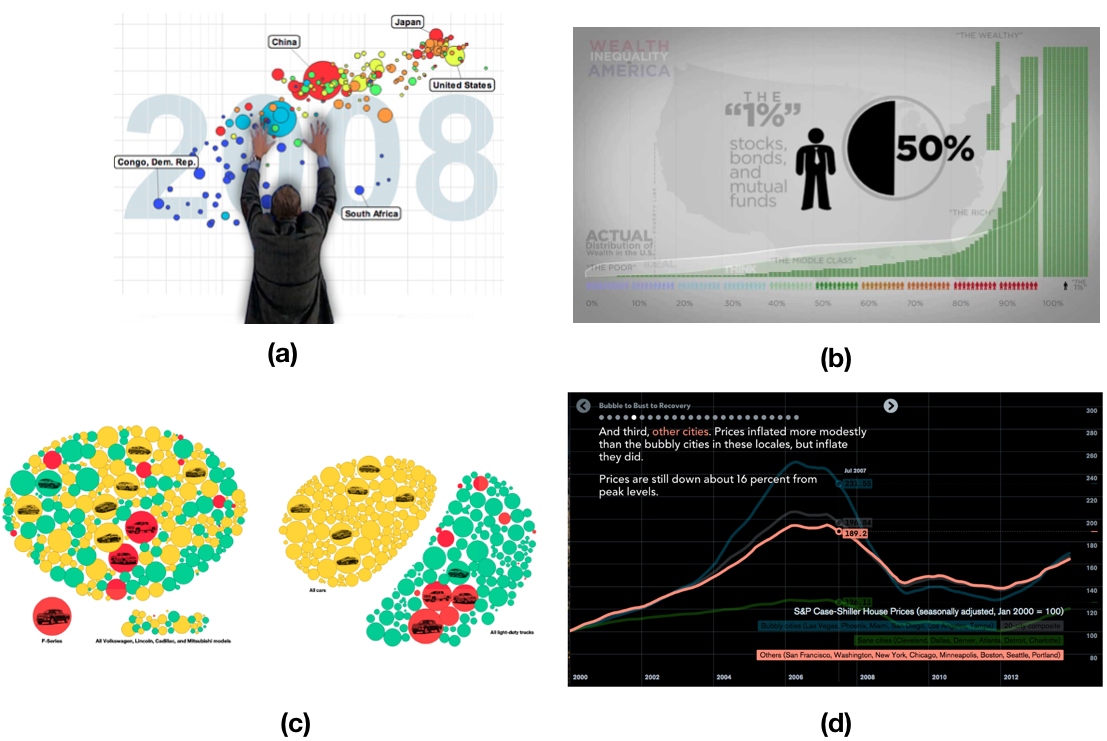
\includegraphics[width=0.95\textwidth]{figure/motivation.png} 
	\caption{Different forms of storytelling. Rosling's talk (a) shows trends in human development \cite{gapminder}. A data video (b) reveals wealth inequality in America \cite{inequality}. Online interactive  visualizations from Bloomberg tell stories such as \textit{Addicted to Trucks} (c) \cite{trunks} and \textit{Bubble to Bust to Recovery} (d) \cite{bust}.} 
	\label{motivation} 
\end{figure}

The current research into data visualization has attached importance to exploratory data analysis. Many visual analytics systems aim to provide novel interfaces and interactions for data exploration, and some also integrate advanced machine learning and data mining algorithms to support powerful analysis ~\cite{May2010}. Comparatively less attention has been paid to the communication function of visualization. However, with the increasing roles of visual data-driven stories and interactive visualization in data analysis, this line of research is attracting interest. The Dagstuhl seminar held in 2016 ~\cite{Carpendale2016} invited both researchers and practitioners to dig into the topic of storytelling using visualization.  Microsoft launched the "data-driven storytelling" project ~\cite{Microsoft}, which aims to understand the story design process and explore methods for easy creation. In spite of several breakthroughs in this field, there is still a plethora of research remaining to be done. For example, although some work ~\cite{Amini2015, Stolper2016, Segel2010} has identified a variety of techniques from existing stories, there is a lack of guidance on how to organize  these techniques given a specific topic. In addition, how to evaluate the effectiveness of not only visual data stories but also visualization authoring tools is yet an open question.


\section{Challenges}
Storytelling is considered as the next step for visualization, specifically for it can present data in an interpretable way ~\cite{Kosara2013}. Thus, we have naturally come to issues of effective visual design in data-driven storytelling. In reference to the design implications informed by good graphics ~\cite{Tversky2002}, visual  design in data-driven narratives should better conform to these two principles as well: one focuses on the content and form of the representation and the other pays attention to the comprehension and perception of the viewers. Therefore, we present three primary challenges resulting from the representation and evaluation of stories, and the limits of authoring tools. 

The first challenge is how to tell stories clearly with engaging visual effects. On the one hand, the mission of a data story is to get a point across and to have the audience understand and trust the content ~\cite{Kosara2013}. Neither describing data and generating insights from an existing dataset nor arranging them in an interpretable way is an easy task.
On the other hand, attractive visual effects contribute to a good narrative. A typical approach is to gain empirical knowledge from a curated collection of data stories. However, the derived design guidance is incomprehensive and constantly evolving. The way to inform an appropriate design space is still under explored.
%Fortunately, storytelling works in a variety of disciplines, leading to theories and practice to produce such effects. It brings a huge opportunity for us to borrow from other fields. However, the way to embed these effects into visual data stories is still under explored.


The second challenge is how to evaluate the effectiveness of such visual data stories. While many interesting stories are widespread and well received in the online media such as Gapminder ~\cite{gapminder} and US wealth inequality ~\cite{inequality}, there is a lack of clearly defined metrics or evaluation methods. Typical measures used in visualization mostly consider time spent on given tasks and their response accuracy through a user study. Nevertheless, these are not pertinent to storytelling, which, instead, requires a crucial evaluation of comprehension, engagement, and memorability of viewers. It also gives rise to problems about comparing the effectiveness of different storytelling techniques. 


Finally, the third challenge is how authoring tools could help support visual narrative designs and lower the barriers to craft data stories. Creating data stories is never a trivial task, relying on a broad set of tools and skills. Authors are expected to use dedicated software or even do the programming themselves when constructing a complete story. Existing tools are limited in many aspects. For example, professional softwares such as Adobe Illustrator or After Effects have steep learning curves and require users' capabilities to design and generate materials. Lightweight tools with a focus on single functions ask for extra tools to complete a story. It is challenging to strike a balance between design flexibility and efficiency of authoring tools. 


\section{Overview}
There are many research issues for transforming data into visually shared stories. However, in this survey, we do not intend to use the term "storytelling" in a broad way that considers all data visualizations as stories. Specifically, this survey mainly focuses on a narrow definition of a visual data story ~\cite{Lee2015}. For example, we exclude exploratory data analysis visualizations which allow users to explore freely and interactively but provide little guidance. In addition, visualizations without enough annotations or written explanations can hardly be considered as well-told stories, since they require viewers to interpret the contents themselves.  Therefore, our analysis is based on asynchronous stories with some form of author-specific narration. Our goal in thie paper is twofold: 1) to review what makes a compelling visual data story based on three primary story components; 2) to investigate ways to author narrative visualization. The rest of this survey is organized as follows.


In Chapter \ref{sec-taxonomy}, we introduce some existing taxonomies for narrative visualization and visual storytelling. After that, we describe our taxonomy derived from the definition of the term "narrative". 


In Chapter \ref{sec-design}, we further illustrate how the visual design in data-driven narratives are developed based on three story components, namely, scenes, sequences, and connection, thus informing the design space. Various techniques are applied in different components to compose compelling and interpretable visual data stories. We then attempt to identify and categorize the design features with collected visualizations.


In Chapter \ref{sec-tool}, we investigate tools to help construct data-driven stories and discuss the evaluation methods used in these visualization authoring tools. 
%Specifically, according to the automatic degree, there exist three kinds of methods to generate visual narrative designs, that is, automatic generation, semi-automated algorithms, and authoring tools.

% In Chapter 4, we categorize core visual narratives based on the surveyed literature from both computer science research and data visualization practice. Particularly, visual narratives mainly facilitate data-driven storytelling in the aspects of trends, ranks, comparisons, relationships, and map presentation.

Finally, we 
%summarize  design implications regarding existing works in Chapter \ref{sec-implication}, and 
conclude some future research directions of visual  design in data-driven narratives in Chapter \ref{sec-conclusion}. 


\newpage

\chapter{Taxonomy}\label{sec-taxonomy}
In this chapter, we first introduce two existing taxonomies given by Segel and Heer ~\cite{Segel2010} and Tong et al. ~\cite{Tong2018}, respectively. The former is a highly cited paper and has contributed greatly to narrative visualization, while the latter is an up-to-date survey on storytelling and visualization adding a variety of new narrative methods and works. We aim to demonstrate their primary characteristics for an overview instead of explaining the technical details of each taxonomy. After that, we propose our taxonomy derived from the definition of the term "narrative". 

\section{Taxonomy by Segel and Heer}

Segel and Heer \cite{Segel2010} investigated 58 examples of narrative visualizations and formulated a design space containing three divisions of features, namely, genres, visual narrative tactics, and narrative structure tactics. 

\begin{figure}[H]
	\centering 
	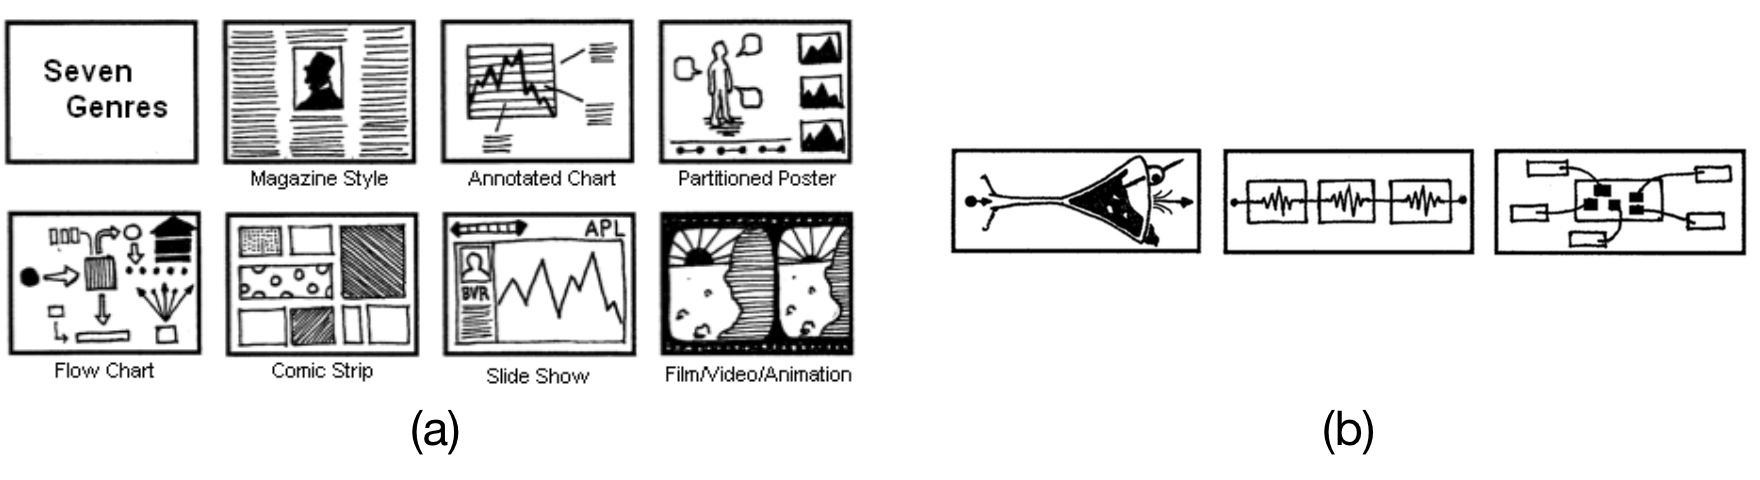
\includegraphics[width=0.9\textwidth]{figure/taxonomy1.png} 
	\caption{(a) Seven genres of narrative visualization. (b) Three schemes of structure. Left: martini glass style; middle: interactive slideshow; right: drill-down story \cite{Segel2010}. } 
	\label{taxonomy1} 
\end{figure}

\begin{compactitem}
	\item \textbf{Genres.} The first division identifies seven basic genres shown in Figure \ref{taxonomy1}(a): magazine style, annotated chart, partitioned poster, flow chart, comic strip, slide show, and film/video/animation.   These genres differ in the number of frames and the ordering of visual elements. 
	
	\item \textbf{Visual Narrative Tactics.} The second division concerns visual mechanisms to facilitate the narrative. These methods are subdivided into three sections. \textit{Visual structuring} describes the way to organize the story and points out the current position of the viewer through visualization (e.g., progress bars). \textit{Highlighting} directs attentions to the emphasized elements using color, motion, etc. \textit{Transition guidance} aims to avoid disorienting the viewer when changing scenes.
	
	\item \textbf{Narrative Structure Tactics.} The third division considers both visual and non-visual techniques to assist the narrative. These ideas are captured in a three-way classification. \textit{Ordering} corresponds to sequences viewers look at through narratives, including linear path, random access, and user-directed path. \textit{Interactivity} allows viewers to manipulate the visualization, while \textit{messaging} displays how visualization communicates insights with viewers combined visual cues and text descriptions (e.g., annotations). 
	
\end{compactitem}

This paper further characterize these design differences in term of the balance between author-driven and reader-driven approaches together with messaging and interactivity. Three common schemes can be classified as shown in Figure \ref{taxonomy1}(b). \textit{Martini glass structure} begins with an author-driven introduction to the narrative, followed by a reader-driven stage to allow interactive exploration. \textit{Interactive slideshow} incorporates interactions within each slide, promoting a dialogue between these two approaches. \textit{Drill-down story} allows readers to choose instances from a given theme, which prioritizes the reader-driven approach.

Though Segel and Heer offered a nice framework and first identified seven genres of narrative visualization, this work is more than 8 years old. The past few years have witnessed some newly emerging formats (e.g., ScrollyTelling \cite{scrollytelling} and SketchStory \cite{Lee2013}) and a gradual shift of existing genres. These changes require a study on recent advancements in narrative visualization. 

\section{Taxonomy by Tong et al.}

Tong et al. \cite{Tong2018} conducted a survey targeting at storytelling literature in visualization, which is much more up to date and shows the evolving field. Besides, instead of a focus on journalism like Segel and Heer \cite{Segel2010}, the authors provided a comprehensive survey of storytelling literature with a coverage of scientific visualization, information visualization, and geo-spatial visualization. 

In this survey, storytelling is considered both as an entity and a creative process. Thus, the taxonomy is first based on the logical notations of who, how, and why. 

\begin{compactitem}
	\item \textbf{Who} plays the main role in storytelling for visualization? This survey identifies two dimensions, namely, \textit{authoring tools} and \textit{user engagement}. The former addresses the author who crafts the story, while the second is about the audience. 
	
	\item  \textbf{How} are stories told? Two categories are classified, i.e., \textit{narrative} and \textit{transition}. Transitions can be further subdivided into animated and static transitions. 
	
	\item \textbf{Why} use storytelling for visualization? \textit{Memorability} and data \textit{interpretation} are important goals for storytelling. They address why authors present data in the form of stories.

\end{compactitem}

The second dimension of this taxonomy refers to the sequence of events, which tracks the viewing path of readers through a narrative. Four categories are extracted. \textit{Linear} indicates that viewers are supposed to follow the order prescribed by the author, while \textit{user-directed path} allows readers to select or create the path. \textit{Parallel} visualizes multiple paths at the same time, and \textit{random access} (also known as \textit{overview}) means no prescribed path. 

The taxonomy in Figure \ref{taxonomy2} presents an overview of important elements in storytelling visualization. However, several dimensions still seem vague and intertwined. For example, as the paper stated itself, "narrative visuals contain the transitions between events", it is hard to distinguish \textit{transition} from \textit{narrative} when categorizing literacy in \textit{how}. In addition, there is no work belonging to \textit{interpretation} in this survey. 

\begin{figure}[H]
	\centering 
	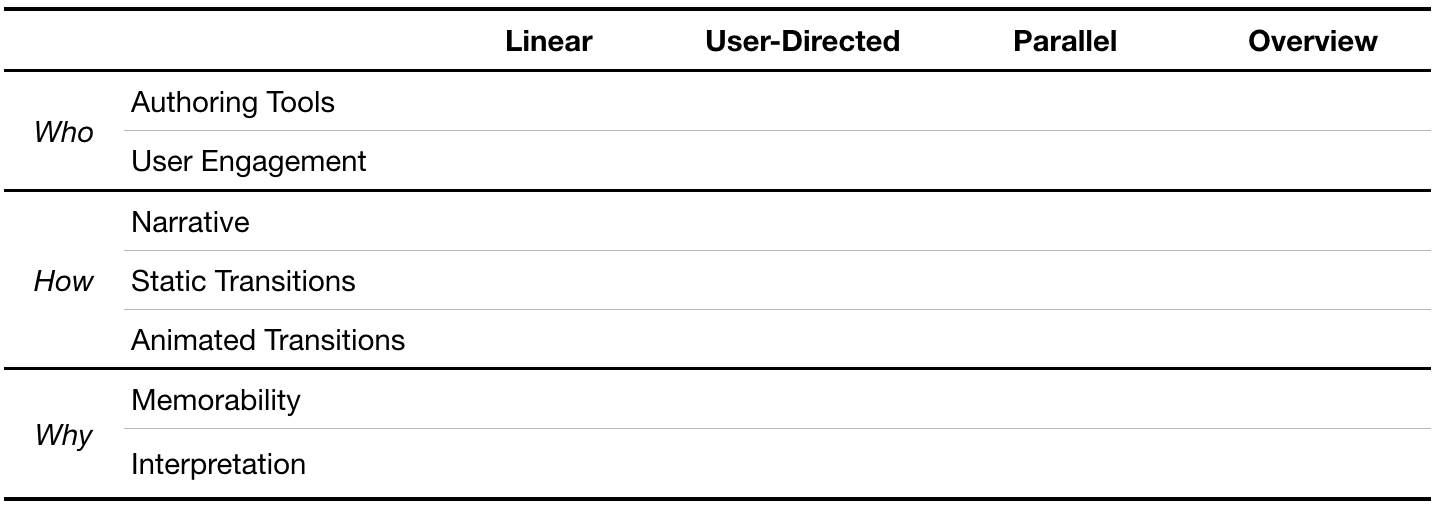
\includegraphics[width=0.95\textwidth]{figure/taxonomy2.png} 
	\caption{ The classification of the storytelling literature proposed by Tong et al. \cite{Tong2018} } 
	\label{taxonomy2} 
\end{figure}

\section{Taxonomy for Visual Design in Data-driven Storytelling}

Segel and Heer \cite{Segel2010} took an empirical approach to investigate the design from an analysis of visualizations. Several works \cite{Bach2018, Stolper2016, McKenna2017} have furthered this line of research and enriched the design space with emerging narrative techniques. However, the capability of visualization practitioners like data journalists to produce artifacts is limited to authoring tools, which did not cover cutting-edge techniques to make compelling stories. Tong et al. ‘s taxonomy did not specify concrete techniques to compose a story. 
%In recent years, we have seen the design space of narrative visualization studied by several academic works as in the above surveys. Most of them \cite{Bach2018, Stolper2016, Segel2010} provided design choices by analyzing existing stories found on popular websites. Since there is a lack of evaluation for the effectiveness of these stories, extracted techniques and their roles in storytelling might not be so faithful and comprehensive.  
Therefore, in this taxonomy, we consider the fundamental components of stories and explore designs with a look into visualization practices and researches. Firstly, in view of the term "narrative", the definition in the Oxford English Dictionary \cite{oed} is "an account of a series of events, facts, etc., given in order and with the establishment of connections between them". Following this explanation, we propose our taxonomy for visual design in data-driven narratives, which consists of three components.


\begin{compactitem}
	\item \textbf{Scene}. The "scene" component concerns the explanation of data and the communication of messages. \textit{Visualization types} work closely in conjunction with data. Despite diverse custom visualizations depending on different tasks, a few types appear frequently, e.g., maps, bar charts, and pictographs. \textit{Textual annotation} includes descriptions beyond and on visualization, which assists both in narration and interpretation. \textit{Highlighting} performed by changing graphical properties or leveraging close-up techniques draws readers' attention to the emphasized elements.
	
	\item \textbf{Sequence}. The second component reflects on the author-specific ordering in storytelling, which imposes a structure to a story and enhances the navigation for readers. \textit{Linear} narratives are typical in data-driven storytelling. \textit{Non-linear} narratives are well received in movies, which shed light on the design of visual data stories. 

	\item \textbf{Transition}. The third component links separate story scenes with attractive visual effects. To convey a story smoothly, many techniques are explored such as camera motions, temporal and spatial controls, animated transtions, morphing, and metaphors. 
\end{compactitem}

Our taxonomy tries to better explore and summarize the content and representation of each story component. Thus, it could facilitate visualization selections. The organization of a story is somehow analogous with PowerPoint slides: each scene can be considered as a slide; the sequence indicates how authors organize multiple scenes or slides in a certain order; and the transitions are similar to visual effects when switching from one slide to another. Actually, some works, especially surveys, may address more than one theme. We have to recognize subjectivity when categorizing a diverse set of designs into a taxonomy and placing them by what we determine to be the main focus of the work. The detailed visual design techniques are described in Chapter 3.


\newpage
% !TeX spellcheck = <none>
\chapter{Visual Narrative}\label{sec-design}
Given the proliferation of data-driven storytelling in practice, it is of great importance to advance researches in visualization to identify factors that make visual data stories compelling and improve their performance in return. This chapter introduces existing works that focus on visual design in data-driven narratives. According to the role each work mainly serves in the storytelling process, we divide them into three categories, namely, scene, sequence, and transition. Considering a well-known principle in the design field, namely, "form follows function" \cite{form}, we then discuss main forms of visual narrative design and their corresponding functions in each category as shown in Table \ref{tab:story-component}. The representative works are describe in detail with both benefits and drawbacks. 
%In each category,we then describe the representative works in detail and discuss their benefits and drawbacks. 
%Based on this taxonomy, we also analyze a sample of existing visual data stories collected from online sources in Table []. 
Based on this taxonomy, we review current visualizaiton genres and  reflect on how they compose a visual data story.

\renewcommand{\arraystretch}{1.5}

\begin{table}[H]
	\centering
	\begin{tabular}{|l|c|l|l|}
		\hline
		\multicolumn{2}{|l|}{Categories}                                                                          & Form                        & Function                                                                             \\ \hline
		\multirow{13}{*}{\begin{tabular}[c]{@{}l@{}}Story\\ Component\end{tabular}} & \multirow{5}{*}{Scene}      & Close-up,~\cite{Furnas1986}                    & \multirow{2}{*}{Highlight}                                                           \\ 
		&                             & Change graphical properties~\cite{Waldner2014} &                                                                                      \\ \cline{3-4} 
		&                             & Text~\cite{Hullman2013, Gao2014, Ren2017}                        & Annotation                                                                           \\ \cline{3-4} 
		&                             & Pictogrphics~\cite{Goffin2017, Wang2018}                & Visual                                                                               \\ \cline{3-4} 
		&                             & Scale~\cite{Qu2018}                       & Consistency                                                                          \\ \cline{2-4} 
		& \multirow{3}{*}{Sequence}   & Timeline~\cite{Brehmer2017}                    & Navigation                                                                           \\ \cline{3-4} 
		&                             & Linear narrative,~\cite{Hullman2013a, Hullman2017, Kim2017a}            & \multirow{2}{*}{Structure}                                                           \\ 
		&                             & Non-linear narrative~\cite{Bach2018, Kim2018}        &                                                                                      \\ \cline{2-4} 
		& \multirow{5}{*}{Transition} & Camera motions~\cite{Wijk2004},              & \multirow{5}{*}{\begin{tabular}[c]{@{}l@{}}Linking\\ separated\\ scenes\end{tabular}} \\ 
		&                             & Static transition ~\cite{Robertson2008},           &                                                                                      \\ 
		&                             & Animated transition~\cite{Chevalier2014, Dragicevic2011, Elmqvist2008a, Guilmaine2012, Heer2007, Plaisant2002},         &                                                                                      \\ 
		&                             & Morphing~\cite{Drucker2015},                    &                                                                                      \\ 
		&                             & Metaphor~\cite{Huron2013, Lin2013, Wang2016},                    &                                                                                      \\ \hline
	\end{tabular}
\caption{Visual design in data-driven storytelling. In the \textit{Form} column, we list forms used in the related papers. The \textit{Function} column list the role the corresponding form serves.}
\label{tab:story-component}
\end{table}

%\renewcommand{\arraystretch}{1.3}

%\begin{table}[H]
%	\centering
%	\begin{tabular}{ |c|c|c|p{15em}|p{7.5em}| } 
%		\hline
%		\multicolumn{3}{|c|}{Categories} & Form & Function \\
%		\hline
%		\multirow{15}{6em}{\centering Story Component} & \multicolumn{2}{|c|}{\multirow{5}{6em}{\centering Scene}}
%		& Close-up, & \multirow{2}*{Highlight} \\
%		& \multicolumn{2}{|c|}{} & Change graphical properties & \\ 
%		\cline{4-5}
%		& \multicolumn{2}{|c|}{} & Text Narration  & Annotation \\ 
%		\cline{4-5}
%		& \multicolumn{2}{|c|}{} & kNNs & instance-based \\ 
%		\cline{2-5}
%		& \multicolumn{2}{|c|}{\multirow{5}{6em}{\centering Sequence}}
%		& Decision Trees, & \multirow{3}*{simplification} \\
%		& \multicolumn{2}{|c|}{} & Sparse SVMs , & \\
%		& \multicolumn{2}{|c|}{} & Sparse CNNs  & \\
%		\cline{4-5}
%		& \multicolumn{2}{|c|}{} & Sparsity by Bayesian , & \multirow{2}*{direct-sparsity} \\
%		& \multicolumn{2}{|c|}{} & Integer Models & \\
%		\cline{2-5}
%		& \multicolumn{2}{|c|}{\multirow{5}{6em}{\centering Transition}}
%		& Decision Trees, & \multirow{3}*{rule-based} \\
%		& \multicolumn{2}{|c|}{} & Rule Lists , & \\ 
%		& \multicolumn{2}{|c|}{} & Rule Sets & \\ 
%		\cline{4-5}
%		& \multicolumn{2}{|c|}{} & Linear Models  & linear \\ 
%		\cline{4-5}
%		& \multicolumn{2}{|c|}{} & kNNs & instance-based \\ 
%		\cline{2-5}
%		\hline
%	\end{tabular}
%	\caption{Visual design in data-driven narratives.}
%	\label{tab:story-component}
%\end{table}

\section{Scene}
One of the important components in data-driven storytelling is visual design in scenes, which aims to communicate events and facts in conjunction with data to a broad audience. Qualified visual representations are supposed to describe data and amplify cognition. With a curated collection of visualization artifacts online, some researchers conducted surveys to extract techniques and inform the design space.

Segel and Heer ~\cite{Segel2010} took an initial step in classifying techniques and formulating the design from an analysis of 58 examples, as was mentioned in Section 2.2. This kind of work has shed light on further research in narrative visualization. Hullman and Diakopoulos ~\cite{Hullman2011} expanded their discussion including extra-representational influencers like contextual differences in interpretation. They distinguished four editorial layers for conveying meaning, which covered the whole creation process from the data, visual representation, textual annotation, to interactivity. Based on an observation of 51 professionally-produced narrative visualizations, five major forms of rhetorical techniques were identified in this genre of storytelling, namely, information access rhetoric, provenance rhetoric, mapping rhetoric, procedural rhetoric, and linguistic rhetoric. Specifically, these strategies of visualization rhetoric worked as an analytical framework to understand how visual techniques could prioritize particular interpretations. Since then, Stolper et al. ~\cite{Stolper2016} also adopted this empirical approach to enrich the range of techniques in constructing scenes, such as textual and audio narration, text annotation, labeling, and tooltips, and show their evolution over time. While many of these surveys investigate data stories but are agnostic to the data type, Brehmer et al. ~\cite{Brehmer2017} provided a detailed analysis which is specific to timelines describing from three dimensions, namely, representation, scale, and layout. Thus, several fundamental elements embellishing scenes have been recognized through multiple iterations, such as annotations, representation, and highlights.

Although extracting design guidance by empirical studies is deemed as a feasible approach, it faces several problems.  The design knowledge is derived from a small sample of visualization examples and is also continually evolving, thus leading to the incompleteness \cite{Moritz2018}. And there exists inevitable subjectivity when grouping and summarizing techniques. Apart from conducting surveys to inform the design space, the visualization research community has proposed new methods to optimize the scene representations recently. 

Nearly all the above surveys argued that text \textbf{annotations} play an important role in supplementing visualization and directing readers' attention. Many efforts have been made to create annotated information visualizations for online news \cite{Hullman2013, Gao2014}. Hullman et al. \cite{Hullman2013} proposed the Contexifier system targeting at providing context for business news as shown in Figure \ref{Contexifier}. It first automatically creates a timeline graph of one company’s stock. Other articles with relevant contents about this company feed information to the additive customized annotations for the line graph visualization. The selection and layout of those annotations in the graph depended on an underlying algorithm in view of three factors, namely, linguistic relevancy of the topic, visual saliency based on the data series, and analysis of article volume about historical events. 

\begin{figure}[htb]
	\centering 
	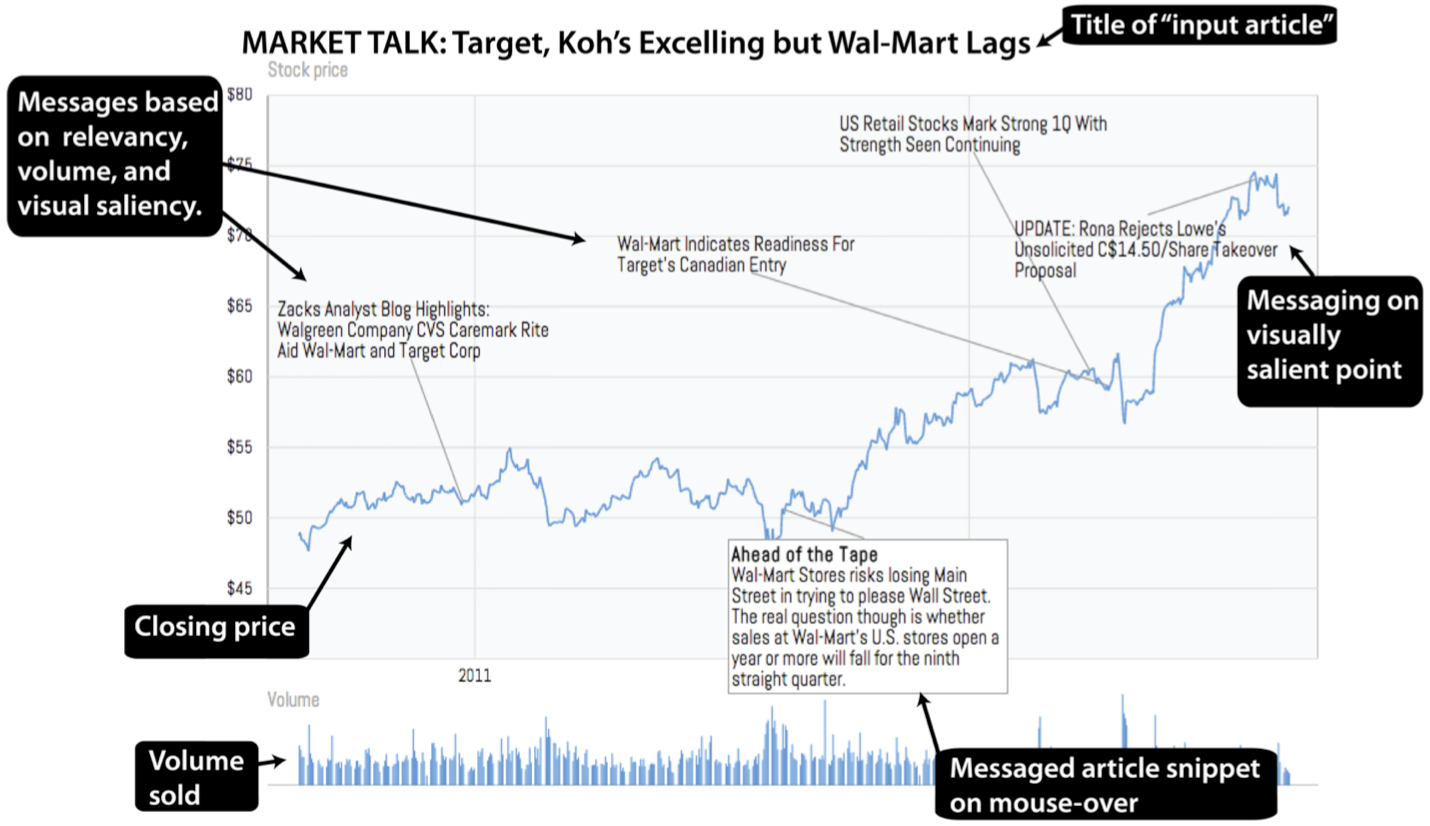
\includegraphics[width=0.95\textwidth]{figure/contiexifier.png} 
	\caption{ An annotated visualization produced by Contextifier \cite{Hullman2013}. } 
	\label{Contexifier} 
\end{figure}

Since Contextifier takes a step towards annotated news visualization but is limited to the stock time series using line charts, Gao et al. \cite{Gao2014} further contributed a news generation pipeline to this area. 
%As shown in Figure \ref{pipeline}, this pipeline negotiated six main points based on an abundant news corpus. 
And the NewsView system implemented this pipeline to automatically generate interactive and annotated maps, which was the most prevalent form of these visualization. 

In addition to automated generation, Ren et al. \cite{Ren2017} developed ChartAccent, an authoring tool that allows users to augment charts with annotations easily. The current system provided manual and data-driven annotations based on the design space informed by 106 annotated charts. However, the problem in the reproduction study is that default data-driven annotations were not ideal most times. It reflects on the challenge that the initial design space might be incomprehensive, leading to the ineffectiveness of the tool.

Among a variety of narrative visualizations, most rely on a few basic visualization forms, such as the above line graphs, bar charts, and maps, as well as \textbf{infographics} (also known as pictographs) \cite{Amini2015}. Some researches \cite{Amini2018} also attest to the prominence of pictographic representation by triggering viewers' engagement compared with standard charts through a crowd-sourced online study. Therefore, it attracted research interests in easing the creation of data-driven infographics \cite{Kim2017, Wang2018} and embedding them to provide compelling scenes \cite{Amini2017, Goffin2017}.

\begin{figure}[htb]
	\centering 
	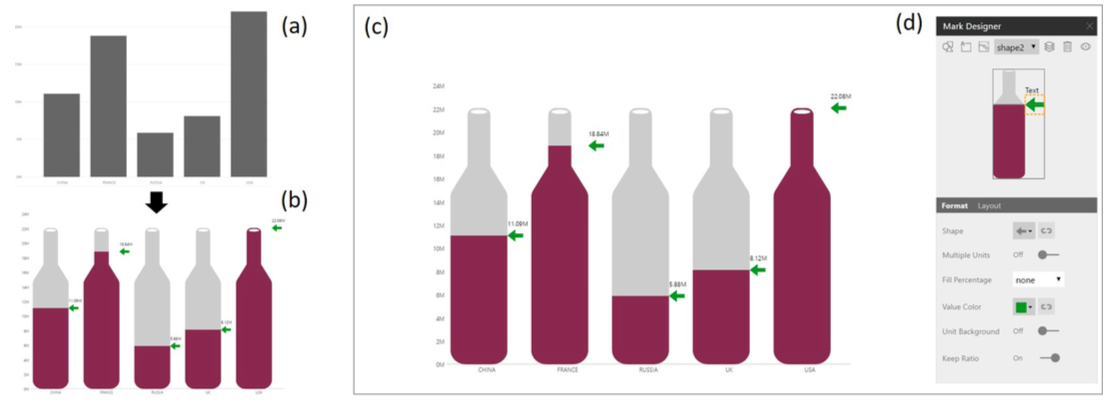
\includegraphics[width=0.98\textwidth]{figure/InfoNice.png} 
	\caption{A use case to change the original column chart to an infographic style version with customized marks with InfoNice \cite{Wang2018}. } 
	\label{InfoNice} 
\end{figure}


Another frequent technique adopted by authors when creating scenes is to perform element \textbf{highlighting}.  There are many methods found in visualization practices, such as wrapping highlighted items with a shape and fading out unessential parts to emphasize important ones. 
Waldner et al. \cite{Waldner2014} enhanced the focus to pop out from its context in a large dynamic scene using a strong visual attractor, flicker. Some movie narrative techniques could be used for reference in data-driven storytelling. For example, fisheye views \cite{Furnas1986} as a close-up highlight element details to the audience. 

Despite these promising design guidelines, an often-overlooked aspect is the wide existence of multiple views. Effective single views may constitute inconsistent multiple scenes, leading to slow and error-prone interpretation. Qu and Hullman presented a qualitative study to investigate specific \textbf{consistency} constraints and exceptions \cite{Qu2018, Qu2016}. As shown in Figures \ref{Consistent}, there were more validations than exceptions considering constrains specialized to scales (e.g., color scale, x or y scale).  The exceptions indicated conditions where specific design rationales should defend inconsistencies and override constraints. These findings provided a foundation for automated inconsistency detection mechanisms. Nevertheless, this work mainly started   from the perspective of authors to create multiple scenes and did not study the impacts inconsistency leave to viewers. 

\begin{figure}[htb]
	\centering 
	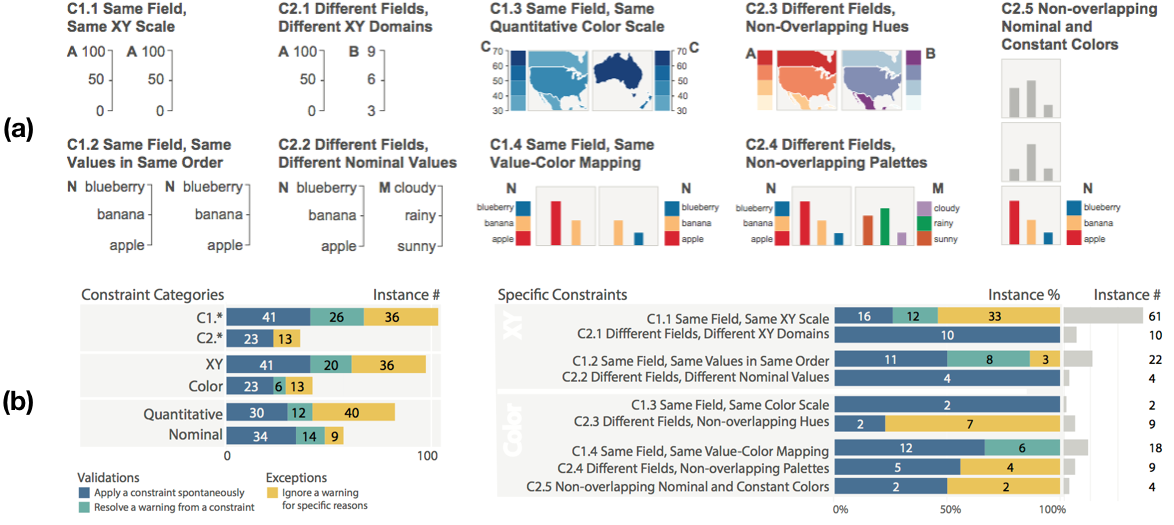
\includegraphics[width=0.98\textwidth]{figure/consistent1.png} 
	\caption{Qu and Hullman conducted quantative studies for XY and color scales to investigate consistency principle (a) and counted validation and exception (b) \cite{Qu2018}. } 
	\label{Consistent} 
\end{figure}


In summary, many surveys have identified basic elements and techniques from analysis of visualization artifacts. Several works develop tools to either ease the creation or augment representations. And the research community also begins to explore high-level design principles such as consistency to further embellish storytelling. However, the expressiveness and effectiveness are evaluated based on a small sample of both users and visualizations in most cases. And there remain research efforts to explore more design considerations. For example, audio narration like background music is indispensable in some narrative forms, but few works have advanced in this direction.

\section{Sequence}

Conveying a narrative with data visualization requires story creators to thread representations into a compelling yet understandable sequence. This form of author-specified ordering differentiates itself from open-ended explorations by providing navigation aids frequently with explicit structures. Several surveys ~\cite{Stolper2016, Segel2010} initialize and further enlarge a variety of techniques used in visualization artifacts to communicate structures and navigation to viewers. These techniques include next/previous buttons, scrolling, breadcrumbs, section header buttons, menu selection, timelines, and geographic maps. Besides, some works focus on the narrative structures. Based on Cohn's theory of visual narratives ~\cite{Cohn2013}, Amini et al. ~\cite{Amini2015} identified the structures from a qualitative analysis of 50 data videos, which consisted of four major narrative categories, i.e., Establisher (E), Initial (I), Peak (P), Release (R). An example with detailed explanation for each category is shown in Figure \ref{sequence1}. According to the findings, they noted that most data videos followed this method, and the Initial category played the most prominent role in data videos. 

\begin{figure}[htb]
	\centering 
	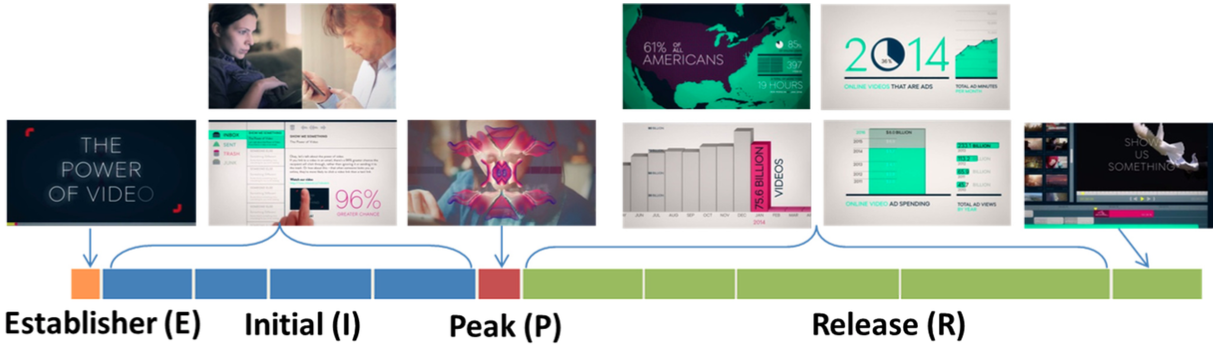
\includegraphics[width=0.98\textwidth]{figure/sequence1.png} 
	\caption{Visual narrative structures: \textit{Establisher} provides referential information; \textit{Initial} "sets the action or event in motion"; \textit{Peak} reflects on the most important events; and \textit{Release} shows "the aftermath of the Peak" \cite{Amini2015}. } 
	\label{sequence1} 
\end{figure}

Researches in the visualization community have studied this category in depth. Hullman et al. ~\cite{Hullman2013a} provided a deeper understanding of sequence in the form of linear, "slideshow-style" presentations. Starting from a qualitative analysis of 42 narrative visualizations, they gained insights on how to structure visualization storytelling. The first finding pointed out six transition types distinguished by changes to data dimensions and used to drive transformations between visualizations.  Another finding describes higher-level strategies that local transitions (visualization-to-visualization) respond to a small number of changes to data dimensions, while global transitions (involving multiple local transitions) are required to maintain consistency in the form of parallelism. These results helped them build a semi-automatic graph-driven approach for visualization sequence supports. An objective function is proposed with an aim to minimize the transition costs considering audience's perceptions. After that, Hullman et al. ~\cite{Hullman2017} further studied impacts that transitions bring to longer visualization sequences. Their results indicated a hierarchical structure preferred by humans beginning with grouping subsets of visualizations with shared data properties.

Based on these works, Kim et al. ~\cite{Kim2017a} presented GraphScape, a directed graph model to extend automated reasoning about visualization similarity and sequencing. Instead of a focus on conceptual transition types as Hullman et al. did, GraphScape leverages the Vega-Lite language and works on a more sophisticated cost function balancing local and global transitions. Thus, this model works both as a generative tool (e.g., given a started visualization, traverse the graph and provide a sequence for this series of visualizations) and an evaluation tool (e.g., given a sequence of visualizations, measure their costs). However, this work currently implements at a level of visualization specification and does not go deep into the data level. 

\begin{figure}[htb]
	\centering 
	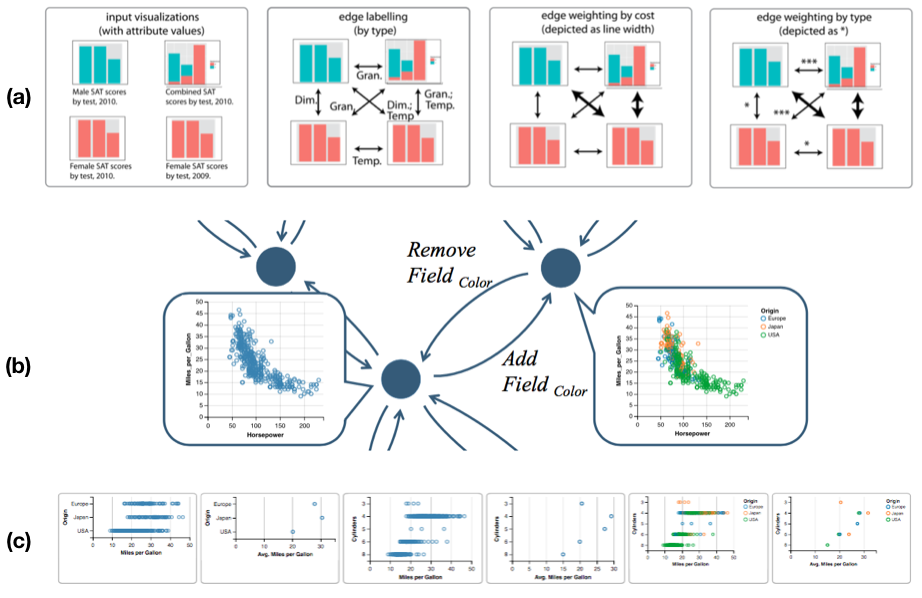
\includegraphics[width=0.98\textwidth]{figure/GraphScale2.png} 
	\caption{ (a) Diagram of the graph-based approach where each visualization represents a nodes and edges stand for possible transitions whose weights are calculated by the cost function \cite{Hullman2013a}. (b) The GraphScape model extended from (a) \cite{Kim2017a}. (c) An example of a viusalizaion sequence. } 
	\label{GraphScale} 
\end{figure}

However, above works all focus on linear sequences. In practice, narrative visualizations do not necessarily conform to the linear narration. For example, a well-received data video named "Wealth Inequality in America" ~\cite{inequality} does not adopt a linear narrative as well. It is based on comparisons among three conditions, i.e., the ideal condition, what American think, and the reality. Recently, Kim et al. ~\cite{Kim2018} presented Story Explorer to visualize non-linear narratives in movies. It provided a curated collection of non-linear narrative techniques, including flashbacks, flashforwards, bidirectional flashes, zigzags, follow-the-hero, and so on. Bach et al. \cite{Bach2018} identified flashback as a critical narrative in data comics. Wang et al. \cite{Wang2016} applied foreshadowing to present video clickstream data. However, most of them are not studied in the field of data-driven storytelling and few tools support to embed these techniques for visualization sequencing.

\section{Transition}

A narrative typically contains an account of multiple events or facts described in a series of ordered scenes. Linking these separated story scenes is crucial, especially providing transitions with attractive and engaging visual effects. Segel and Heer ~\cite{Segel2010} pointed out \textit{transition guidance} as an important dimension in visual narrative tactics. They found the common techniques in narrative visualization borrowed from films, e.g., camera motions, animated transitions. As such, much practice and research have studied this category in depth.  

\textbf{Camera motions} remain an ever-present mechanism in many visual data stories. The main advantage of imagining a virtual camera in data-driven narratives is its innate nature, as it conforms to the way how humans perceive the real world. Thus, it can easily elicit viewers' engagement by triggering their emotions. For example, in the "Global Wealth Inequality" video \cite{globalnequality}, when describing the richest 1\% have accumulated 43\% of our world's wealth, the authors moved the camera quickly along the bar but still took some time to reach the top. It easily provoked emotions and emphasized the wealth gap between the rich and the poor to the audience. In addition to camera viewing, other techniques such as zooming and panning are used frequently as well. Research in this area concentrates more on optimizing the smooth effects and is maturing rapidly.  For instance, Wijk and Nuij \cite{Wijk2004} presented a model to handle smooth viewing with a focus on simultaneous zooming and panning. However, the evaluation of the effect was based on the perception and did not consider the cognitive aspects which also played an important role in this kind of animation. 

\begin{figure}[htb]
	\centering 
	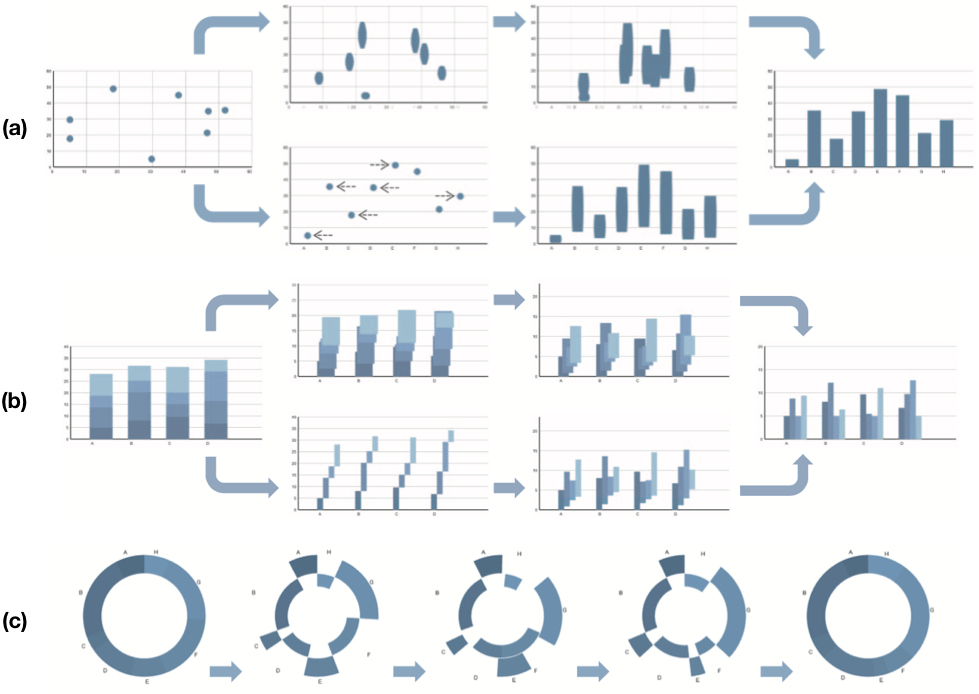
\includegraphics[width=0.98\textwidth]{figure/transition.png} 
	\caption{ Animated transitions between statistical data graphics. (a) Animating from a scatter plot to a bar chart. (b) Animating from stacked bars to grouped bars. (c) A multi-stage animation of changing values in a donut chart \cite{Heer2007}. } 
	\label{animated} 
\end{figure}

\textbf{Animated transitions} are another promising technique to connect story scenes and facilitate perception of changes between related data visualizations.  As a typical example like \textit{Green Honey} \cite{honey} shows, when viewers scroll down, the transitions will be triggered by small points' flying to their new position according to different colors. Heer and Robertson \cite{Heer2007} studied the design and effectiveness of animated transitions between statistical data visualizations such as bar charts, pie charts, and scatter plots as shown in Figure \ref{animated}. They crafted a taxonomy of seven transition types and proposed a visualization system, DynaVis for assessing the efficacy. The finding showed that animated transitions can improve graphical perception. However, not all animated transition scenarios are significantly different. For example, staged transitions only gain modest performance compared with linear transitions. Also, in this work, they just identified the design space among three common statistical data graphics and did not cover a wide range of transition scenarios. Some researches expand it to tree structures. Plasisant et al. \cite{Plaisant2002} proposed SpaceTree breaking the transition into 3 stages. Guilmaine et al. \cite{Guilmaine2012} further compared four animated transitions in a radial tree visualization, i.e., linear, staged, hierarchical, and a hybrid animation mixed with the staged and hierarchical approaches. The results indicate the hierarchical transitions in tree visualizations outperform other techniques significantly. However, the evaluation was just based on a target-tracking task and required to be further validated. Another research focus on animated transitions is to evaluate the effectiveness of  such techniques like temporal distortion \cite{Dragicevic2011} and staggering effects \cite{Chevalier2014} in visual tracking. The findings showed the benefits using these techniques, but the extent depended on the conditions and transition types.

Besides, animated transitions in \textbf{3D space} is much eye-catching. Some software like PowerPoint and Keynote has already embedded such transitions such as cube and box. Elmqvis et al. \cite{Elmqvist2008a} integrated animated rotations in 3D space, somewhat akin to rolling the dice, in scatterplot matrix navigation. 

\textbf{Morphing} is a special effect in animations which "changes one shape into another through a seamless transition" \cite{morphing}. This technique has been applied to several online visual data stories, such as EPFL Data Monolith \cite{EPFL} and The Rhythm of Food \cite{food}. They typically use points as basic elements. The previous data graphic is separated into multiple points, then these points animate to their new positions and form a new data visualization. Similarly, Drucker and Fernandez \cite{Drucker2015, Park2018} presented SandDance to explore the effectiveness of animating between unit representations as shown in Figure \ref{sandDance}.  

\begin{figure}[H]
	\centering 
	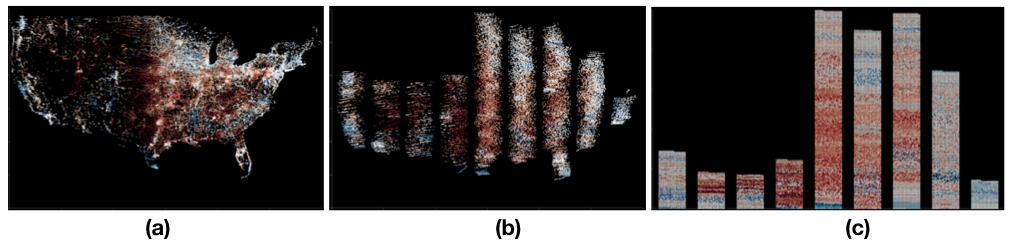
\includegraphics[width=0.98\textwidth]{figure/SandDance.png} 
	\caption{ A sequence explores the 2010 American election \cite{Drucker2015}. (a) Scatter plots are colored by voting percents on the map. (b) The path interpolates between the starting and ending states. (c) Bar charts are binned by logitude. } 
	\label{sandDance} 
\end{figure}

\textbf{Visual metaphors} show wonderful performance in data-driven storytelling and presentation but require much creativity. Visual Sedimentation \cite{Huron2013} presents an attractive design metaphor for visualizing data streams in Figure \ref{sedimentation}. It simulates the real-world sedimentation processes where objects fall because of gravity and then aggregate into strata over time. As for data streams which have incoming data continually, sedimentation fits a lot since data is encoded as objects and a force model controls the falling rate. Wang et al. \cite{Wang2016} also used this metaphor to visualize video clickstream data. Lin and Vuillemot \cite{Lin2013} explored spirograph designs for ambient display of Tweets. However, one problem for these visual metaphors is that they increase pressure for viewers to accurately extract the data. It might be not appropriate for strict data exploration.

\begin{figure}[htb]
	\centering 
	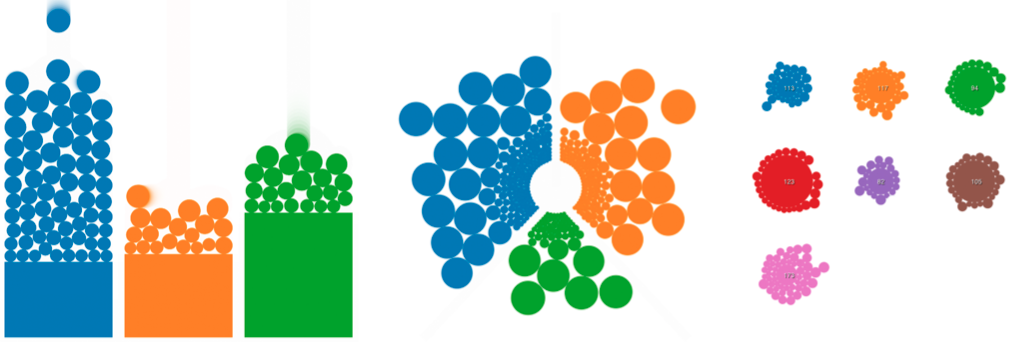
\includegraphics[width=0.95\textwidth]{figure/sedimentation.png} 
	\caption{ The Visual Sedimentation metaphor is applied to a bar chart (left), a pie chart (center), and a bubble chart (right) \cite{Huron2013}. } 
	\label{sedimentation} 
\end{figure}

Despite multiple animated transition techniques have been created and implemented in the visualization research, Amini et al. \cite{Amini2017} found such transitions are uncommon in data videos today. They suspected the complexity of realizing them with some programming skills and the lack of support in existing video editing tools contribute to the deficiency. Thus, they opted to support such kind of transitions as shown in Figuire \ref{lens}. However, they only extended  chart transitions \cite{Heer2007} to and from pictographs. Their finding  also indicated a gap that data visualization tools are not keeping up with the pace of innovations, as Google News Lab pointed out \cite{GoogleNews}. 

\begin{figure}[htb]
	\centering 
	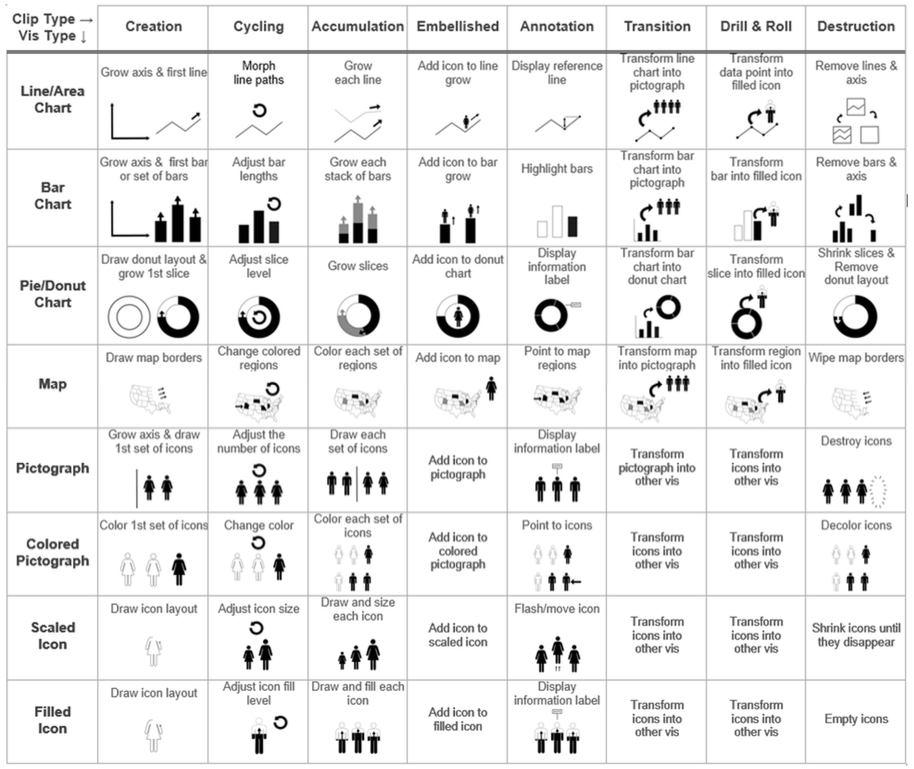
\includegraphics[width=0.95\textwidth]{figure/lens.png} 
	\caption{ Clip types as a function of  visualization types (rows)  and animation types  (columns) supported by DataClips \cite{Amini2017}. } 
	\label{lens} 
\end{figure}

However, the use of animation always arouses a heated discussion \cite{Fisher2010}. Robertson et al. \cite{Robertson2008} compared two alternative trend visualizations based on static representations in Figure \ref{trend} with the animated Gapminder Trendalyzer. The finding showed that trend animation can be challenging both in analysis and presentations. Although animations made participants enjoyable and exciting, it resulted in many errors. However, some works \cite{Amini2018, Heer2007} argued that animation can boost understandability of data insights and increase focused attention. Thus, without a series of unified evaluation criteria, it is hard to assess the effectiveness of visual data stories.

\begin{figure}[htb]
	\centering 
	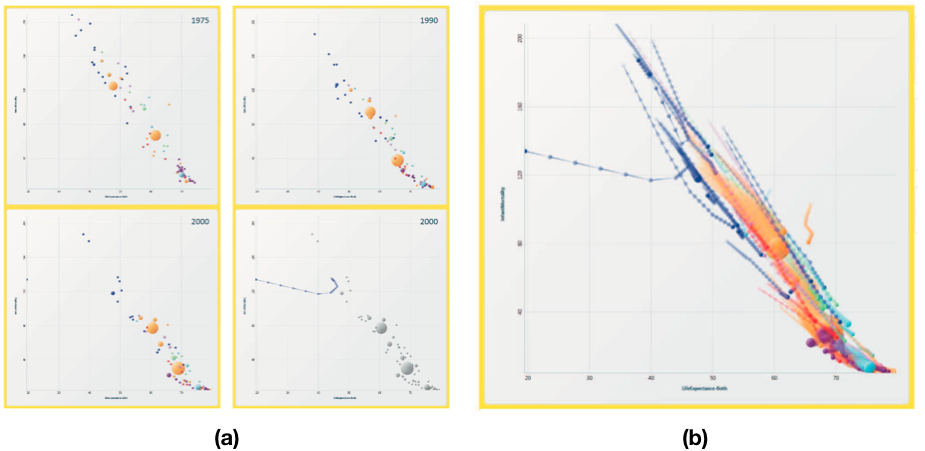
\includegraphics[width=0.95\textwidth]{figure/Trend.png} 
	\caption{ Two alternative static trend visulizations \cite{Robertson2008}. (a) A small multiples display the trend traces side by side. (b) One display shows traces of all trends overlaid simultaneously. } 
	\label{trend} 
\end{figure}


\section{Combining Multiple Components}

In the above sections, we identify three major components to compose a data-driven narrative, namely, scenes, sequences, and transitions. We learn from both research and practice to inform the design space of each component, respectively. Actually, a visual data story is not required to explicitly comprise all three parts. Take seven genres of narrative visualization (Figure \ref{taxonomy1}) for example. A magazine style which embeds visualization in a page of text or an annotated chart usually has a single frame. Thus, they may clearly address the scene design. The sequence and transition deal more with external factors such as text narration. Authors may consider the narrative sequence for the layout of partitioned posters ("multi-view visualizations"), flow charts, or comic strips, but are likely to employ a simple static transition between multiple frames. When authoring slide shows or film, these three components all play important roles. The scene design gives a basic representation to communicate data insights. The narrative sequence works for the goal of storytelling such as comparisons and trends, thus amplifying cognition. Advanced animated transition effects engage a broad range of viewers.

We also examine the story components with new emerging genres like ScrollyTelling \cite{scrollytelling} and SketchStory \cite{Lee2013}. First, ScrollyTelling asks viewers to scroll down to explore visual stories. It is similar to slide shows but provide more transition techniques such as scrolling interactions and animation effects. SketchStory spans annotated charts, partitioned posters, and videos. It allows authors to sketch along the real-time presentation with pen and touch interactions as shown in Figure \ref{sketchStory}. It enriches the storytelling with audio narration and real-time feedback.

\begin{figure}[htb]
	\centering 
	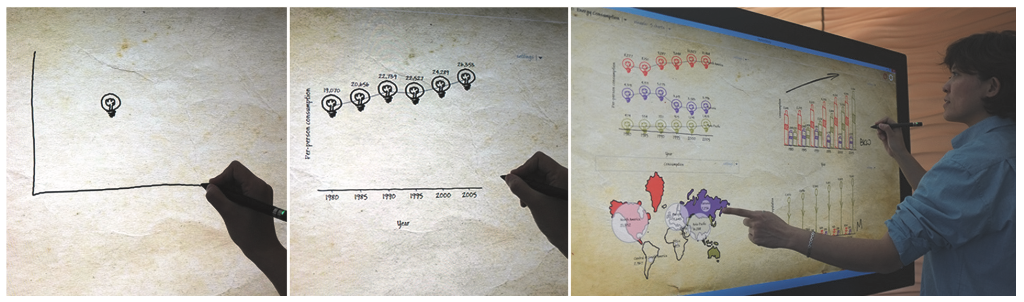
\includegraphics[width=0.95\textwidth]{figure/SketchStory.png} 
	\caption{ Telling a real-time story using SketchStory \cite{Lee2013}. } 
	\label{sketchStory} 
\end{figure}

However, we have seen that the proliferation of different narrative visualization genres and richness of techniques they employ in practice are largely limited to the authoring tools. Many research works have developed novel design and interactions. Most of them are not embedded into existing tools and require extra programming capabilities which practitioners tend not to equip with. 


\newpage
\chapter{Narrative Authoring Tools}\label{sec-tool}

As summarized at the end of Chapter 3, by learning from strategies used in practice and reflecting on the problems when crafting stories, the research community has devoted great efforts to building tools that help users to easily visualize data and communicate narratives. However, with the proliferation of narrative authoring tools, it arouses another challenge to evaluate and compare the strengths and weakness among these tools. A feasible approach is to adjust the different evaluation standards from the perspective of the research contribution. Therefore, in this chapter, we review the related narrative authoring tools with regards to their contributions, evaluation criteria, and evaluation methods in detail, and discuss the research opportunities concerning different parts.

\section{Approaches}

Different approaches feature prominently in tools intended to craft data-driven narratives. The approach selection is closely related to the contribution of the tool. In the following, we give an overview of existing tools that facilitate storytelling.

\subsection{Automatic Generation}
Automatic tools can be found in the applications of annotations and presentation orders. Contextifier \cite{Hullman2013} and NewsViews \cite{Gao2014} are both used to construct annotated visualization in news to contextualize text articles. Some works \cite{Hullman2013a, Kim2017a} leverage the directed graph model to automatically reason visualization sequencing in a linear order. However, no existing tool could craft a rich data story automatically. Most of them augment the storytelling in a specific element to some extent. This form provides hints for tool builders to determine which element in data-driven narratives could be improved by automatic generation and which asks for human-in-the-loop tools. 

\subsection{Authoring tools}

There already exists a multitude of general-purpose tools to create data graphics or videos, such as Adobe Creative Suite, Microsoft Excel and Power BI. However, most of them have a steep learning curve and are difficult for users to manipulate data directly. Thus, crafting data-driven narratives is much time-consuming with these tools. 

Recent narrative authoring tools \cite{Amini2017, Satyanarayan2014} are more expressive and efficient with a curated collection of visual design choices. For example, Satyanarayan and Heer \cite{Satyanarayan2014} instantiated a storytelling model in Ellipsis, which provides an interface for users to add elements to augment data storytelling in visualization. Amini et al. \cite{Amini2017} implemented DataClips, an authoring tool to craft a complete data video with a library of data-driven clips. These clips contain popular visualization types with corresponding animation types and can be easily extended to new clips. Some dedicated tools are built for specific storytelling elements. For instance, ChartAccent \cite{Ren2017} aims to support data-driven annotation. InfoNice \cite{Wang2018} enables easy creation of data-driven infographics. A list of narrative authoring tools with their major functions is summarized in Table \ref{tab:authoring-tool}. However, the proliferation of narrative authoring tools brings about difficulties and challenges for users to select the appropriate tool and evaluate its effectiveness. 

\subsection{Programming}

It is certainly possible to craft narrative visualization by programming. Actually, many computer science researchers work on this way and also provide a large palette of open-source libraries and packages, such as D3.js, processing, and Vega. Notably, there even exist libraries specific to some function, e.g., swoopyDrag.js or labella.js for data-driven annotation and labelling, and anime.js for animation. Iterative design between creating visualization with D3 and editing it with Illustrator is doable as well with the Hanpuku bridge tool \cite{Bigelow2017}. However, although these programming languages lend much freedom to customize data-driven narratives precisely, many visualization practitioners like data journalists are not equipped with capable programming skills. They require an interactive interface to author the story directly and intuitively. Therefore, many research efforts concentrate on developing better tools to ease the creation.

\section{Evaluation Criteria}

Actually, information visualization evaluation always presents difficulties and has been discussed frequently among the research community. Many works \cite{Plaisant2004, Lam2012} contribute to establishing a series of evaluation criteria and methods. The BELIV workshop series focuses on the challenges of evaluation in visualization. However, the evaluation targeting at narrative authoring tools faces another obstacle. For example, typical evaluation is based on controlled experiments to compare users' performance such as completion time and error rates. But it is challenging to assess these criteria in view of an authoring system which supports users' creative work. It is hard to calculate time and errors for a visual story creation. What's more, the primary problem is the lack of an appropriate comparative system. Most of novel authoring systems are designed and developed due to the insufficient functions of existing systems. It is reasonable that the newly-developed tool should outperform the existing one. However, users must have the diverse knowledge of tools. Like, a professional Adobe Illustrator designer gets accustomed to using this software but may not have enough time to learn the full capacities of the new authoring system, where the tutorial is mostly limited to a short study session. It brings difficulties to control essential factors and set tasks during the evaluation experiment. Therefore, a series of evaluation criteria is required to guide the approach.

Amini et al. \cite{Amini2018a} recently proposed a variety of criteria to consider when evaluating a narrative authoring tool. It is natural that the list does not cover an exhaustive set of criteria. It still sheds light on our thinking. We propose a tailored list of criteria combined with their work and evaluation standards derived from the previous survey of relevant tools. And with an increasing trend of narrative authoring tools in the future, the study of criteria for evaluating data-driven storytelling tools will grow at length. Currently, they can be grouped to eight aspects as follows. 

\begin{compactitem}
	\item \textbf{Expressiveness}.  The tool provides with a number of design choices, including various visualization types, annotation, and interactions. Users are allowed to create a range of possible visual data stories with the system.

\item \textbf{Flexibility}. It relates to the extent to which an author can extend the given library of design choices and make custom designs. This criterion demands a balance between creative work and ease of creation. 

\item \textbf{Guidance}. Some tools target at novice users who are likely to have problems when creating stories. It would be of great help to provide design support such as making layout suggestions during the process. 

\item \textbf{Efficiency}. It concerns the speed to produce a data-driven story using the tool, i.e., users can create how many stories within the limited time. This criterion is of great importance to some kinds of users such as journalists who need to produce stories frequently and quickly. 

\item \textbf{Usability}. Given an expected data-driven story, the tool should provide a series of functions for users to craft it.

\item \textbf{Learnability}. The learning curve of the storytelling tool are closely related to the number of functions and intuitive interactions the tool provides. Qualified documents and abundant tutorial materials can also help ease the learning. 

\item \textbf{Integration}. An authoring tool for narrative visualization is supposed to be integrated into current workflow and assist in authors' creative work. This criterion asks tool builders to understand the methods authors are using to create data-driven stories.

\item \textbf{Iteration}. The process to craft a data-driven story inevitably involves several iterations. It assesses the extent to which the tool supports iterative controls.

\end{compactitem}

Actually, a qualified narrative authoring tool is not necessarily required to satisfy all of these criteria. Good tool designers should strike a balance and make trade-offs among these criteria when they build such tools. Suitable evaluation standards should depend upon the research contribution that the system intends to achieve. For example, if the contribution of a tool is to help automatically construct annotated visualizations to contextualize data-rich texts (e.g., \cite{Hullman2013}), flexibility may be not adopted for the evaluation. But when the system aims to allow users to realize a broad range of designs (e.g., \cite{Wang2018}), the evaluation should attach great importance to the expressiveness criterion. 

\section{Evaluation Methods}

Ren et al. \cite{Ren2018} discussed the evaluation methods used in many visualization authoring systems whose main research contribution lies on “expressive” designs. They summarized six approaches to conduct evaluation in these works. We, here, mainly follow their methodology but just focus on storytelling tools as discussed in Section 4.1. Since general visualization authoring systems do not necessarily equip with the capability of storytelling, they mostly provide visualization for data exploration and analysis like Microsoft Excel. Authors need to edit the generated visualization with other tools to support narratives. Although some tools like DataInk \cite{Xia2018} focus on binding data with Information graphics, their main contribution lies on creative design not data-driven storytelling. Notably, we include InfoNice \cite{Wang2018}, because it is incorporated into an analytics tool, bridging the gap between data exploration and presentation. Another exception is SketchStory \cite{Lee2013}, which allows presenters to freeform sketch on a digital whiteboard  during the process. Therefore, we summarize the evaluation methods of narrative authoring tools in Table \ref{tab:authoring-tool}, which is different from the one of Ren et al. in some aspects. 

\begin{table}[H]
	\centering
	\begin{tabular}{|c|c|c|c|c|c|c|}
		\hline
		& Approaches  & \begin{tabular}[c]{@{}c@{}}Empirical\\ Study\end{tabular} & \begin{tabular}[c]{@{}c@{}}Reproduct\\-ion Study\end{tabular} & \begin{tabular}[c]{@{}c@{}}Free-Form\\ Study\end{tabular} & \begin{tabular}[c]{@{}c@{}}Comparative\\ Study\end{tabular} & Gallery    \\ \hline
		Contextifier\cite{Hullman2013}                                                   & automated   & survey                                                    &                                                              &                                                           & y                                                           &            \\ \hline
		NewsViews\cite{Gao2014}                                                      & automated   & survey                                                    &                                                              &                                                           &                                                             &            \\ \hline
		Sequence\cite{Hullman2013a}                                                       & automated   & survey                                                    &                                                              &                                                           &                                                             &            \\ \hline
		GraphScape\cite{Kim2017a}                                                     & automated   &                                                           &                                                              &                                                           &                                                             &            \\ \hline
		DataClips\cite{Amini2017}                                                      & authoring   & survey                                                    &                                                              & y                                                         & video design                                                &            \\ \hline
		ChartAccent\cite{Ren2017}                                                    & authoring   & survey                                                    & y                                                            &                                                           &                                                             &            \\ \hline
		\begin{tabular}[c]{@{}c@{}}Timeline\\ Storyteller\cite{storyteller}\end{tabular} & authoring   & survey                                                    &                                                              &                                                           &                                                             &            \\ \hline
		Ellipsis\cite{Satyanarayan2014}                                                       & authoring   & interviews                                                &                                                              & y                                                         &                                                             & y          \\ \hline
		InfoNice\cite{Wang2018}                                                       & authoring   &                                                           &                                                              &                                                           & y                                                           & y          \\ \hline
		SketchStory\cite{Lee2013}                                                    & authoring   & \begin{tabular}[c]{@{}c@{}}wizard-of\\ -oz\end{tabular}   & y                                                            & y                                                         & y                                                           &            \\ \hline
		Hanpuku\cite{Bigelow2017}                                                        & program &                                                           &                                                              &                                                           &                                                             & 3 cases \\ \hline
	\end{tabular}
	\caption{Evaluation methods used for each of the narrative authoring tools. "y" means the evaluation method was conducted for this tool. }
	\label{tab:authoring-tool}
\end{table}

\subsection{Empirical Study}
Brehmer et al. \cite{Brehmer2014} introduced empirical study in a broad way with a multitude of methods, including observational field studies, interviews, and so on. They encouraged pre-design empirical studies for information visualization. One obvious benefit was to characterize work practices and associated problems, thus informing the design space. In the data-driven storytelling field, many works present exemplary instances through a pre-design empirical study. A favorite way is to analyze a curated collection of existing stories. For example, Brehmer et al. first surveyed 263 timelines and identified 14 design choices with three dimensions \cite{Brehmer2017} to build Timeline Storyteller \cite{storyteller}. Amini et al. \cite{Amini2015} attained empirical knowledge with two exploratory studies. The first was to identify high-level structures with key components based on a qualitative examination of 50 online data videos through the cinematography lens. Then, they observed the creation process of 13 experienced storytellers. The derived design space worked as the cornerstone for DataClips \cite{Amini2017} they developed for authoring data videos. Another way to understand empirical knowledge is to involve end users. For example, Satyanarayan and Heer \cite{Satyanarayan2014} conducted formative interviews with experienced story makers to learn the general authoring process and limitations of current tools. SketchStory \cite{Lee2013} conducted a Wizard of Oz study and usage tests with participants \cite{Walny2012} to iterate the design.

In summary, when designing authoring tools, empirical studies play a critical role both in informing design spaces and justifying trade-offs. They provide an initial understanding about the tool framework. 

\subsection{Reproduction Study}
In a reproduction study, participants are asked to reproduce a copy of the given visual data stories. This study is often served as a tutorial to familiarize subjects with the authoring tool, which first examines its learnability. ChartAccent \cite{Ren2017} and SketchStory \cite{Lee2013} both featured a reproduction study. It should be noted that this study can encounter the usability issues. For example, participants complained that ChartAccent \cite{Ren2017} didn’t support z-order manipulation. SketchStory \cite{Lee2013} iterated the system design after the reproduction study and free-from study.

However, the main weakness is that a reproduction study does not conform to the reality. Such tools are built to support creative work and author novel data-driven narratives. The finding from a reproduction study can not totally demonstrate the usability.

\subsection{Free-Form Study}
A free-form study requires participants to author their own visual data stories with the tool. DataClips \cite{Amini2017}, Ellipsis \cite{Satyanarayan2014}, and SketchStory \cite{Lee2013} all utilized this evaluation. This study simulates the real-world usage scenario and can be used to assess multiple aspects of the authoring tool, such as expressiveness, learnability, and usability. In this experiment, it should be noted that there is likely to be a phase before creation for users to get familiar with data and facts \cite{Amini2017}, as well as generate and sketch ideas \cite{Lee2013}. 

However, a free-form study tends to last limited time duration. That means the participants may not have enough time to master all functions the tool provides, as well as create a variety of visualization artifacts. Therefore, the expressiveness can’t be demonstrated fully in this study.

\subsection{Comparative Study}
Tool builders are likely to conduct a controlled experiment to compare their tools with existing commercial software tools. It can be used to highlight the usability and efficiency. For example, Wang et al. compared InfoNice \cite{Wang2018} with Data-Driven Guides \cite{Kim2017} and measured time to create an infographic-style visualization with the same data using these two tools. Lee et al. \cite{Lee2013} employed SketchStory to do real-time presentations as compared to the traditional way using PowerPoint. They measured the engagement for both the audience and presenter and found sketching facilitate storytelling in that scenario. Amini et al. \cite{Amini2017} asked participants to create data video using DataClips against the combination of Adobe Illustrator and Adobe Effects, because there was no such similar tool to craft data videos directly. Thus, it brings a problem that the experiment is not under strict controls. It is hard to find an appropriate evaluation matrix to compare tools accurately. We have remarked that research prototypes contribute to novel features and may not incorporate some engineering functions such as “undo/redo”. However, in practice, these functions do work. Thus, it may decrease the impression among participants and also increase the creation time in the comparative study. 

\subsection{Gallery}
As we have mentioned in Section 4.3.3, subjects can only master limited capability to show expressiveness of the tool in limited time. Researchers recently have thought to provide a gallery themselves to demonstrate expressiveness. Ellipsis \cite{Satyanarayan2014}, InfoNice \cite{Wang2018}, and Hanpuku \cite{Bigelow2017} all offer galleries for review. The benefits are obvious in expressiveness and efficiency.  However, a major concern might be the target users can’t produce such visualization artifacts as the authors do. Detailed tutorials and instruments should be complemented. Since the gallery is provided by the tool builder, it can not show the usability and learnability of tool. It is supposed to be combined with other evaluation methods. 


 \newpage


\chapter{Conclusion and Future Work}\label{sec-conclusion}
The emergence and fast development of web-based visualization technologies paves the way for a proliferation of online visual data-driven stories. In this survey, we review visual design in data-driven storytelling and also pay attention to tools that facilitate authoring visual data stories. After introducing two taxonomies respectively based on narrative genres and storytelling roles in visualization, we organize our taxonomy based on three primary components to guide visual design in composing data-driven narratives. Then we investigate narrative authoring tools to assist in crafting high quality visualization artifacts and reflect on methodologies adopted to evaluate these tools.


The research in data-driven storytelling is a growing discipline. There is a large palette of visual data storytelling techniques emerging and recurring in a multitude of forms ranging from animated infographics and videos to interactive online visualizations. However, visualization tools are not keeping up with the pace of innovation. In addition, research on understanding factors to compose high quality data stories should be extended to encompass more advanced techniques, e.g., non-linear narratives and animation. Nowadays, there are efforts being made to understand visual data-driven stories and build narrative authoring tools to facilitate storytelling. We specifically summarize a few challenges and potential research directions which are worthwhile studying further as follows.


\textbf{Understanding of stories.} Some research has demonstrated essential elements of data-driven storytelling. However, most of them analyze explicit techniques, such as text annotations to augment visualization, and timelines or progress bars to provide navigation aids. With visual data stories becoming more abundant and creative, there is certainly room for improvement and new findings. For example, little attempt has been made to understand stories from the perspective of cognitive psychology and perception. How does a compelling story engage a broad audience? Does it ignite emotions among the viewers? If yes, is there any common technique such as visualizing personal data or providing situated design? In addition, few researches have worked on interpreting non-linear narratives and adding audio narration  in data-driven storytelling, whereas many acclaimed data videos or comics \cite{inequality, Bach2018} employ these patterns and convey good stories. How to better incorporate these implicit techniques into the visual design of data-driven stories can be a potential direction for future exploration. 


\textbf{Support from authoring tools.} As mentioned in Section 4, there is an increasing trend of authoring visualization tools, whereas these tools are not keeping pace with innovation. For example, current authoring tools only provide limited animation, which makes it uncommon to see such animated transitions in practice. Besides, they fail to support guidance or warnings during the authoring process. This is mainly due to the incomplete understanding of design choices, like consistency constraints. Another important factor is the end-users who actually craft visual stories for data insight communication. They can be experts or novice users. Thus, different design considerations should be recognized in view of their expertise. For experts, how to integrate these visualization tools into their regular workflows to improve efficiency might be a major concern. While for non-experts, tool builders should provide sufficient tutorials for the use of the tool. Guidance or creation suggestions during the process are welcome as well. 



%%%%%%%%%%%%%%%%%%%%%%%%%%%%%%%%%%%%%%%%%%%%%%%%%%%%%%%%%%%%%%%%%%%%%%%%%
%                                                                       %
%      9) BIBLIOGRAPHY                                                  %
%                                                                       %
% This example uses bibtex to generate the required Bibliography. Refer %
% to the % the file ustthesis_test.bib for the entries of the           %
% Bibliography. Note that only the cited entries are printed.           %
%                                                                       %
% If BibTeX is not used to typeset the bibliography, replace the        %
% following line with the \begin{thebibliography} and \end{bibliography}%
% commands (the "thebibliography" environment) to process the           %
% Bibliography.                                                         %
%                                                                       %
%%%%%%%%%%%%%%%%%%%%%%%%%%%%%%%%%%%%%%%%%%%%%%%%%%%%%%%%%%%%%%%%%%%%%%%%%

%%%%%%%%%%%%%%%%%%%%%%%%%%%%%%%%%%%%%%%%%%%%%%%%%%%%%%%%%%%%%%%%%%%%%%%%%
%                                                                       %
% The recommended bibliography style is the IEEE bibliography style.    %
% "ustbib" defines the IEEE bibliography standard with the added        %
% ability of sorting the items by name of author.                       %
%                                                                       %
% If you are not using BibTeX to process your Bibliography, comment out %
% the following line.                                                   %
%                                                                       %
%%%%%%%%%%%%%%%%%%%%%%%%%%%%%%%%%%%%%%%%%%%%%%%%%%%%%%%%%%%%%%%%%%%%%%%%%

\bibliographystyle{IEEETranS}

\bibliography{ref}
% Please run "bibtex ustthesis_test" before the bibliography can be
% included.

%%%%%%%%%%%%%%%%%%%%%%%%%%%%%%%%%%%%%%%%%%%%%%%%%%%%%%%%%%%%%%%%%%%%%%%%%
%                                                                       %
%     10) APPENDIX (If Any)                                              %
%                                                                       %
% \appendix command marks the beginning of the APPENDIX part of the     %
% Thesis. The usual \chapter command is used for the different chapters %
% of the Appendix.                                                      %
%                                                                       %
%%%%%%%%%%%%%%%%%%%%%%%%%%%%%%%%%%%%%%%%%%%%%%%%%%%%%%%%%%%%%%%%%%%%%%%%%


%%%%%%%%%%%%%%%%%%%%%%%%%%%%%%%%%%%%%%%%%%%%%%%%%%%%%%%%%%%%%%%%%%%%%%%%%
%                                                                       %
%     11) BIOGRAPHY (Optional)                                          %
%                                                                       %
% \biography and \endbiography are used to define the optional          %
% Biography of the author of the Thesis.                                %
%                                                                       %
%%%%%%%%%%%%%%%%%%%%%%%%%%%%%%%%%%%%%%%%%%%%%%%%%%%%%%%%%%%%%%%%%%%%%%%%%

% \biography
% The biography of the student is ALSO optional.
% \endbiography

\end{document}
